% =====================================================================
%  SLIDE BÁO CÁO — Hệ thống nhận diện biển số (Beamer)
%  Biên dịch: XeLaTeX (khuyến nghị) hoặc pdfLaTeX (Overleaf).
%  Cần kèm thư mục docs/images/ để hiển thị hình.
% =====================================================================
\documentclass[aspectratio=169,9pt]{beamer}

\usepackage{iftex}
\ifPDFTeX
  \usepackage[utf8]{inputenc}
  \usepackage[T5]{fontenc}
  \usepackage{lmodern}
  \usepackage[vietnamese]{babel}
\else
  \usepackage{fontspec}
  \usepackage{polyglossia}\setmainlanguage{vietnamese}
  \IfFontExistsTF{DejaVu Sans}{\setsansfont{DejaVu Sans}}{}
  \IfFontExistsTF{DejaVu Serif}{\setmainfont{DejaVu Serif}}{}
\fi

\usetheme{Madrid}
\usecolortheme{whale}
\usepackage{booktabs}
\usepackage{tikz}
\usetikzlibrary{arrows.meta,positioning}
\setbeamertemplate{navigation symbols}{}
\setbeamerfont{frametitle}{size=\large}
\graphicspath{{docs/images/}}

\title[Nhận diện biển số]{Hệ thống nhận diện biển số ứng dụng cho phát hiện phương tiện và đi sai làn}
\subtitle{Báo cáo đồ án môn học --- Thị giác máy tính}
\author[Nhóm VietTraffic]{Hoàng Thị Hoạt \and Đỗ Công Trí \and Nguyễn Đức Mạnh}
\institute[ĐHXD Hà Nội]{Trường Đại học Xây dựng Hà Nội --- Khoa Công nghệ thông tin\\GVHD: GV.\ Nguyễn Đình Quý}
\date{Hà Nội, 2026}

\begin{document}

\begin{frame}[plain]\titlepage\end{frame}

% ---------------------------------------------------------------
\begin{frame}{Đặt vấn đề, mục tiêu và ràng buộc}
\begin{columns}[T]
\begin{column}{0.5\textwidth}
\textbf{Bối cảnh \& thách thức}
\begin{itemize}\footnotesize
  \item Giám sát sai làn tại ngã tư chủ yếu thủ công: tốn người, dễ bỏ sót, thiếu khách quan.
  \item Ảnh camera khó: mờ động, rung, thiếu sáng, biển bị che/bám bụi.
  \item Biển số Việt Nam đa dạng: biển dài/vuông, 4 màu nền, ký tự \texttt{Đ}.
  \item Chỉ sai \textbf{một ký tự} là cả hồ sơ mất giá trị.
\end{itemize}
\end{column}
\begin{column}{0.5\textwidth}
\textbf{Mục tiêu}
\begin{itemize}\footnotesize
  \item Pipeline khép kín: video \(\to\) phát hiện vi phạm \(\to\) đọc biển \(\to\) hồ sơ.
  \item Phát triển mô-đun \alert{OCR tự huấn luyện} (trọng tâm); có demo chạy thực.
\end{itemize}
\smallskip
\textbf{Ràng buộc}
\begin{itemize}\footnotesize
  \item Huấn luyện từ đầu (không pretrained).
  \item Chỉ dùng dữ liệu được cấp.
  \item GPU miễn phí Kaggle T4\(\times\)2.
\end{itemize}
\end{column}
\end{columns}
\end{frame}

% ---------------------------------------------------------------
\begin{frame}{Tổng quan hệ thống \& quy trình}
\begin{center}
\resizebox{0.96\textwidth}{!}{%
\begin{tikzpicture}[font=\scriptsize,
  blk/.style={draw,rounded corners,align=center,text width=2.6cm,minimum height=1.4cm,inner sep=2pt},
  hl/.style={blk,fill=blue!20,line width=1pt},
  arr/.style={-{Latex[length=1.8mm]},thick},node distance=7mm]
  \node[blk](a){Phát hiện \& bám vết\\(YOLOv8m + ByteTrack)};
  \node[blk,right=of a](b){Phân tích sai làn\\(\textit{nếu bật})};
  \node[blk,right=of b](c){Phát hiện biển số\\(YOLO)};
  \node[hl,right=of c](d){Nhận dạng OCR};
  \node[blk,right=of d](e){Lưu trữ \& web\\(FastAPI/SQLite)};
  \draw[arr](a)--(b);\draw[arr](b)--(c);\draw[arr](c)--(d);\draw[arr](d)--(e);
\end{tikzpicture}}
\end{center}
{\scriptsize
\begin{enumerate}
  \item Mỗi khung: YOLOv8m + ByteTrack phát hiện và bám vết xe (trong vùng quan tâm ROI).
  \item Phân tích sai làn theo vùng đa giác (bật/tắt tuỳ chế độ vận hành).
  \item Với xe cần xử lý: nới hộp \(24\%\), dò biển bằng YOLO riêng, chọn khung nét nhất (Laplacian \(\ge 1800\)); lọc trùng (cô-sin \(\ge 0{,}70\)).
  \item OCR đọc biển rồi chuẩn hoá theo luật biển số Việt Nam.
  \item Lưu kết quả vào cơ sở dữ liệu và hiển thị trên web.
\end{enumerate}}
{\footnotesize Hai khối nặng (biển số, OCR) bật/tắt theo \textbf{ba chế độ}: giám sát biển số / sai làn / phạt nguội tích hợp; khối \alert{OCR} là trọng tâm.}
\end{frame}

% ---------------------------------------------------------------
\begin{frame}{Phát hiện \& định vị biển số}
\begin{columns}[T]
\begin{column}{0.45\textwidth}
\begin{center}
\resizebox{!}{0.60\textheight}{%
\begin{tikzpicture}[font=\scriptsize,
  bx/.style={draw,rounded corners,align=center,text width=4.4cm,minimum height=0.7cm,inner sep=2pt},
  arr/.style={-{Latex[length=1.6mm]},semithick},node distance=3.4mm]
  \node[bx](a){Khung hình};
  \node[bx,below=of a](b){YOLOv8m + ByteTrack\\(bám vết trong ROI)};
  \node[bx,below=of b](c){Nới hộp $24\%$ $\rightarrow$ dò biển};
  \node[bx,below=of c](d){Cổng độ nét (Laplacian $\ge1800$)};
  \node[bx,below=of d](e){Chấm điểm + chống trùng};
  \node[bx,fill=blue!12,below=of e](f){Ảnh biển tốt nhất $\rightarrow$ OCR};
  \draw[arr](a)--(b);\draw[arr](b)--(c);\draw[arr](c)--(d);\draw[arr](d)--(e);\draw[arr](e)--(f);
\end{tikzpicture}}
\end{center}
\end{column}
\begin{column}{0.55\textwidth}
\textbf{Quy trình}
\begin{enumerate}\scriptsize
  \item YOLOv8m + ByteTrack bám vết xe, gán \texttt{track\_id} (trong ROI; vết $\ge4$ khung).
  \item Mỗi xe: nới hộp $24\%$ rồi dò biển bằng YOLO riêng (conf 0,25).
  \item Cắt biển, đo độ nét bằng phương sai Laplacian; loại nếu $<1800$.
  \item Chấm điểm chất lượng, giữ khung biển \textbf{rõ nhất} cho mỗi xe.
  \item Chống trùng: cô-sin $\ge0{,}70$, cách $\le110$ px, trong 45 khung.
  \item Đưa ảnh biển tốt nhất sang khối OCR.
\end{enumerate}
\end{column}
\end{columns}
\end{frame}

% ---------------------------------------------------------------
\begin{frame}{Mô hình nhận dạng: kiến trúc \& luồng dữ liệu}
\begin{columns}[T]
\begin{column}{0.56\textwidth}
\begin{center}
\resizebox{!}{0.72\textheight}{%
\begin{tikzpicture}[font=\scriptsize,
  bx/.style={draw,rounded corners,align=center,text width=4.2cm,minimum height=0.7cm,inner sep=2pt},
  hl/.style={bx,fill=blue!15},
  dim/.style={font=\tiny\itshape,inner sep=1pt},
  arr/.style={-{Latex[length=1.6mm]},semithick},node distance=4mm]
  \node[bx](in){Ảnh biển số};
  \node[bx,below=of in](st){CNN Stem (Conv+BN+GeLU+Pool)};
  \node[bx,below=of st](lm){Local Mixing Block};
  \node[bx,below=8mm of lm,xshift=-2.6cm](sq){Gộp chiều cao $\rightarrow$ chuỗi};
  \node[bx,below=8mm of lm,xshift=2.6cm](gp){Global Average Pooling};
  \node[bx,below=of sq](pe){+ Positional Encoding};
  \node[bx,below=of pe](tr){Transformer (8 lớp, 8 heads)};
  \node[hl,below=of tr](ct){CTC Head};
  \node[below=4mm of ct,font=\tiny,align=center](oc){Chuỗi ký tự};
  \node[bx,below=of gp](se){Semantic Head};
  \node[below=4mm of se,font=\tiny,align=center](os){Tập ký tự};
  \node[bx,fill=gray!15,text width=5cm,below=10mm of oc,xshift=2.6cm](loss){Tổng mất mát \emph{(chỉ khi train)}\\ $\mathcal{L}=\mathcal{L}_{\text{CTC}}+0{,}1\,\mathcal{L}_{\text{BCE}}$};
  \draw[arr](in)--(st) node[dim,midway,right]{$48\times192\times3$};
  \draw[arr](st)--(lm) node[dim,midway,right]{$12\times48\times C$};
  \draw[arr](lm.south)--(sq.north);\draw[arr](lm.south)--(gp.north);
  \draw[arr](sq)--(pe) node[dim,midway,right]{$48\times256$};
  \draw[arr](pe)--(tr);
  \draw[arr](tr)--(ct) node[dim,midway,right]{$48\times256$};
  \draw[arr](ct)--(oc) node[dim,midway,right]{$48\times37$};
  \draw[arr](gp)--(se) node[dim,midway,right]{$C$};
  \draw[arr](se)--(os) node[dim,midway,right]{$36$};
  \draw[arr](oc)--(loss);\draw[arr](os)--(loss);
\end{tikzpicture}}
\end{center}
\end{column}
\begin{column}{0.44\textwidth}
\textbf{Lấy cảm hứng từ SVTRv2}
\begin{itemize}\scriptsize
  \item \textbf{Thân chung}: CNN Stem (3$\times$[Conv 3$\times$3+BN+GeLU]+Pool) + Local Mixing (Depthwise Sep.\ Conv + FFN).
  \item \textbf{Nhánh tuần tự} (chính): chuỗi 48 bước, $d=256$, + Positional Encoding $\to$ Transformer 8 lớp $\cdot$ 8 heads (dropout 0,22) $\to$ CTC (37 lớp).
  \item \textbf{Nhánh ngữ nghĩa} (phụ, chỉ train): GAP $\to$ Semantic Head (36), giám sát phụ giúp hội tụ nhanh.
  \item Hai nhánh \textbf{không gộp} đầu ra; chỉ kết hợp ở hàm mất mát. Suy luận chỉ dùng CTC.
  \item Dùng Transformer thay BiLSTM: song song tốt + nắm phụ thuộc tầm xa.
\end{itemize}
\end{column}
\end{columns}
\end{frame}

% ---------------------------------------------------------------
\begin{frame}{Dữ liệu và tiền xử lý}
\begin{columns}[T]
\begin{column}{0.42\textwidth}
\begin{table}\centering\footnotesize
\begin{tabular}{lc}
\toprule
\textbf{Tập} & \textbf{Số ảnh} \\
\midrule
Train & 9.752 \\
Validation & 1.219 \\
Test & 1.219 \\
\midrule
\textbf{Tổng} & \textbf{12.190} \\
\bottomrule
\end{tabular}
\end{table}
{\footnotesize Bộ ký tự: \textbf{36} (0--9, A--Z trừ W, và Đ); thêm \texttt{blank} của CTC \(\to\) 37 lớp.}
\end{column}
\begin{column}{0.58\textwidth}
\begin{itemize}\footnotesize
  \item \textbf{Sửa lỗi mã hoá nhãn} (Mojibake \texttt{Đ/đ}), chuẩn hoá in hoa, xuất CSV.
  \item \textbf{Sinh dữ liệu tổng hợp} \(\times5\) (\(\approx\)58.512 mẫu), giả lập 5 màu biển (trắng/vàng/xanh/đỏ/xanh lá).
  \item \textbf{Tăng cường:} xoay \(\pm3^\circ\)--\(15^\circ\), biến đổi phối cảnh, hạ phân giải, motion/Gaussian blur, nén JPEG (10--35).
  \item \textbf{Phân nhóm đa kích thước}: 40$\times$160, 48$\times$192, 56$\times$224.
\end{itemize}
\end{column}
\end{columns}
\end{frame}

% ---------------------------------------------------------------
\begin{frame}{Chiến lược huấn luyện --- lộ trình tăng tiến}
\begin{table}\centering\footnotesize
\begin{tabular}{p{2.0cm}p{1.4cm}p{4.3cm}p{3.6cm}}
\toprule
\textbf{Giai đoạn} & \textbf{Epoch} & \textbf{Dữ liệu chính} & \textbf{Mục tiêu} \\
\midrule
Nhập môn & 1--40 & Ảnh tổng hợp sạch, augment nhẹ & Học bảng ký tự, cấu trúc \\
Thử thách & 41--160 & Tổng hợp khó (blur, nghiêng) + ảnh thật & Chống nhiễu, mờ, lệch \\
Thực chiến & 161--280 & Tăng tỉ trọng ảnh thật & Tối ưu trên dữ liệu thực \\
Sửa lỗi khó & 281--340 & Lấy mẫu khó & Sửa cặp ký tự dễ nhầm \\
\bottomrule
\end{tabular}
\end{table}
\begin{itemize}\footnotesize
  \item \textbf{Hàm mất mát có trọng số}: phạt nặng ký tự nét mảnh \texttt{1,8,2,3,7,9} (1,8--2,0); giảm số \texttt{0} (0,7).
  \item \textbf{Lấy mẫu khó}: tăng \(\approx45\%\) xác suất xuất hiện các ảnh từng đoán sai.
  \item Thực tế dừng sớm quanh \textbf{epoch 78} (nằm ở giai đoạn 2).
\end{itemize}
\end{frame}

% ---------------------------------------------------------------
\begin{frame}{Chiến lược huấn luyện --- cấu hình \& hội tụ}
\begin{columns}[T]
\begin{column}{0.48\textwidth}
\textbf{Cấu hình (config\_used.json)}
\begin{table}\centering\scriptsize
\begin{tabular}{ll}
\toprule
Optimizer & AdamW \\
Learning rate & \(3\times10^{-4}\) \\
Weight decay & 0,08 \\
Warmup & 2.400 bước \\
Batch size & 128 (DDP, T4\(\times\)2) \\
Dropout & 0,22 \\
EMA decay & 0,9995 \\
Synthetic ratio & 5 \\
\bottomrule
\end{tabular}
\end{table}
\end{column}
\begin{column}{0.52\textwidth}
\textbf{Hội tụ (đơn mô hình)}
\begin{itemize}\footnotesize
  \item Train loss: \(3{,}45 \to 0{,}05\) (epoch 75).
  \item Train exact match: \textbf{95,00\%}.
  \item Val thô (chưa hậu xử lý): \textbf{51,31\%}.
  \item Tốc độ: 87--100 giây/epoch.
\end{itemize}
\smallskip
\footnotesize\alert{Lưu ý:} chênh lệch train 95\% vs val 51,31\% cho thấy \textbf{quá khớp} đáng kể; 51,31\% mới là năng lực thô thực sự.
\end{column}
\end{columns}
\end{frame}

% ---------------------------------------------------------------
\begin{frame}{Kết quả --- số liệu chính (tập Test, 1.219 ảnh)}
\begin{table}\centering\footnotesize
\begin{tabular}{lccc}
\toprule
\textbf{Chỉ số} & \textbf{Mặc định} & \textbf{Quét lại YOLO} & \textbf{Ý nghĩa} \\
\midrule
Character Accuracy & 93,04\% & \textbf{93,06\%} & Tỷ lệ ký tự đúng \\
Full Plate Accuracy & 74,82\% & \textbf{75,39\%} & Đúng 100\% biển \\
Exact Match & --- & 912/1219 & Số biển đúng hoàn toàn \\
Avg Edit Distance & --- & 0,5751 & Số ký tự sửa trung bình \\
Latency (TB / P95) & 74,56 / 136,74 ms & --- & Thời gian/ảnh \\
Throughput & 13,41 ảnh/s & --- & \(\approx\) thời gian thực \\
\bottomrule
\end{tabular}
\end{table}
\begin{itemize}\footnotesize
  \item Tách rõ kết quả \alert{thô} (51,31\% trên val) và \alert{toàn pipeline} (sau hậu xử lý).
  \item Cơ chế quét lại YOLO nâng full-plate từ 74,82\% lên 75,39\%.
\end{itemize}
\end{frame}

% ---------------------------------------------------------------
\begin{frame}{Kết quả --- phân tích lỗi}
\begin{columns}[T]
\begin{column}{0.52\textwidth}
\begin{itemize}\footnotesize
  \item \textbf{Lỗi nhỏ chiếm đa số}: 142 ảnh sai 1 ký tự, 60 ảnh sai 2 ký tự \(\Rightarrow\) ký tự đúng cao nhưng toàn biển thấp hơn.
  \item \textbf{Theo nhóm ảnh}: tốt nhất \texttt{type1} 87,4\%, \texttt{mb} 84,6\%; \alert{khó nhất \texttt{type2} chỉ 54,2\%}.
  \item \textbf{Cặp nhầm phổ biến}: \texttt{4$\to$A} (31), \texttt{0$\to$1} (24), \texttt{0$\to$6} (18), \texttt{T$\to$1} (18), \texttt{T$\to$7} (17).
  \item Nguyên nhân: nét tương đồng, mất viền tròn do mờ, loá sáng.
\end{itemize}
\end{column}
\begin{column}{0.48\textwidth}
\centering
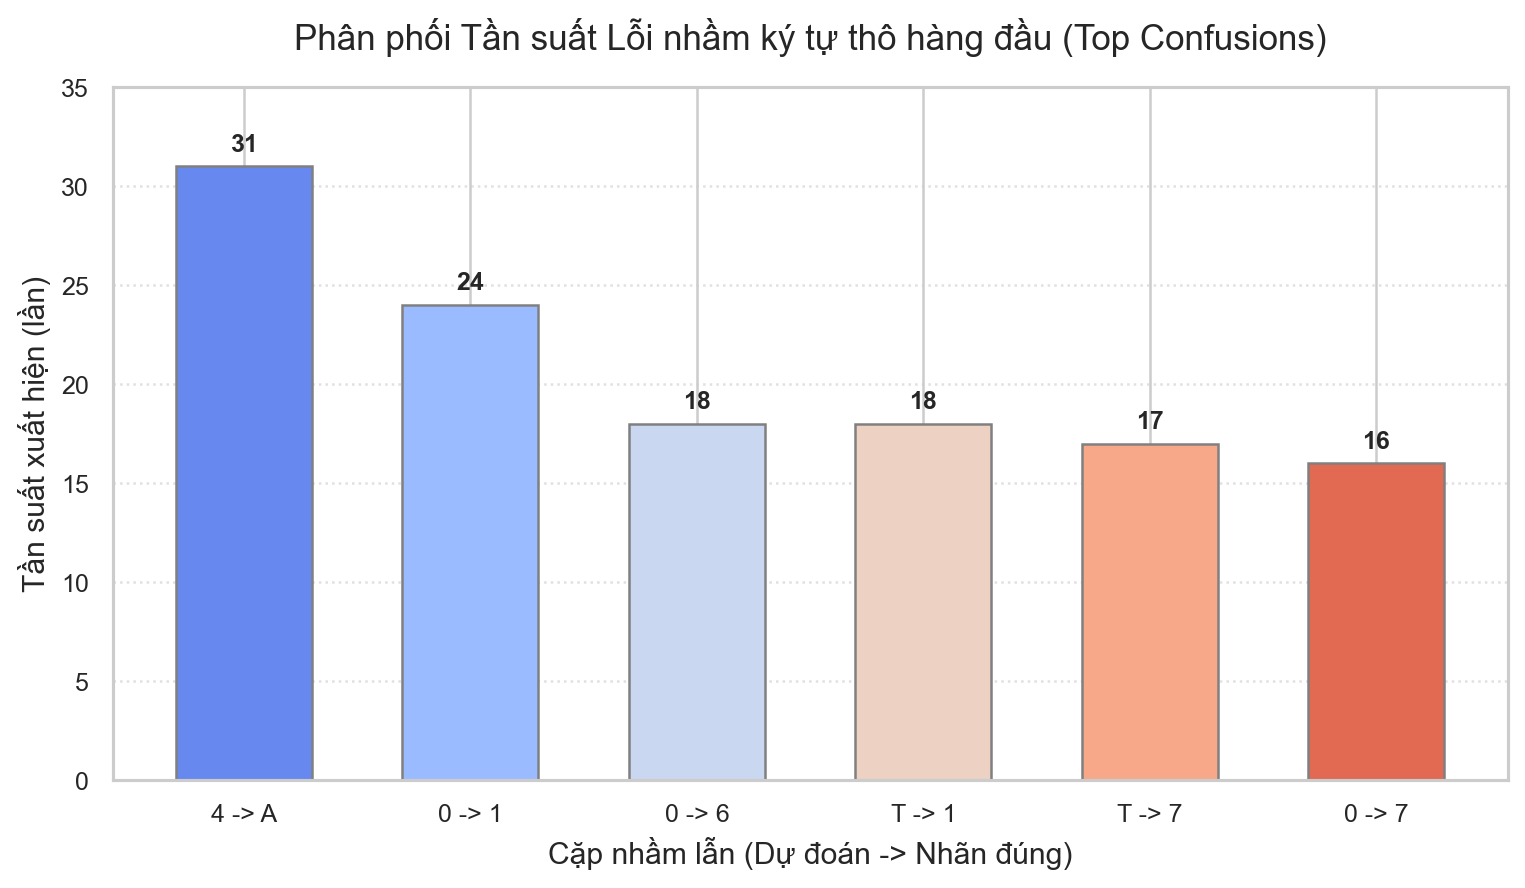
\includegraphics[width=\linewidth]{ocr_character_confusions.png}
\end{column}
\end{columns}
\end{frame}

% ---------------------------------------------------------------
\begin{frame}{Kết quả mô hình \& giao diện kiểm thử}
\begin{columns}[T]
\begin{column}{0.54\textwidth}
\centering
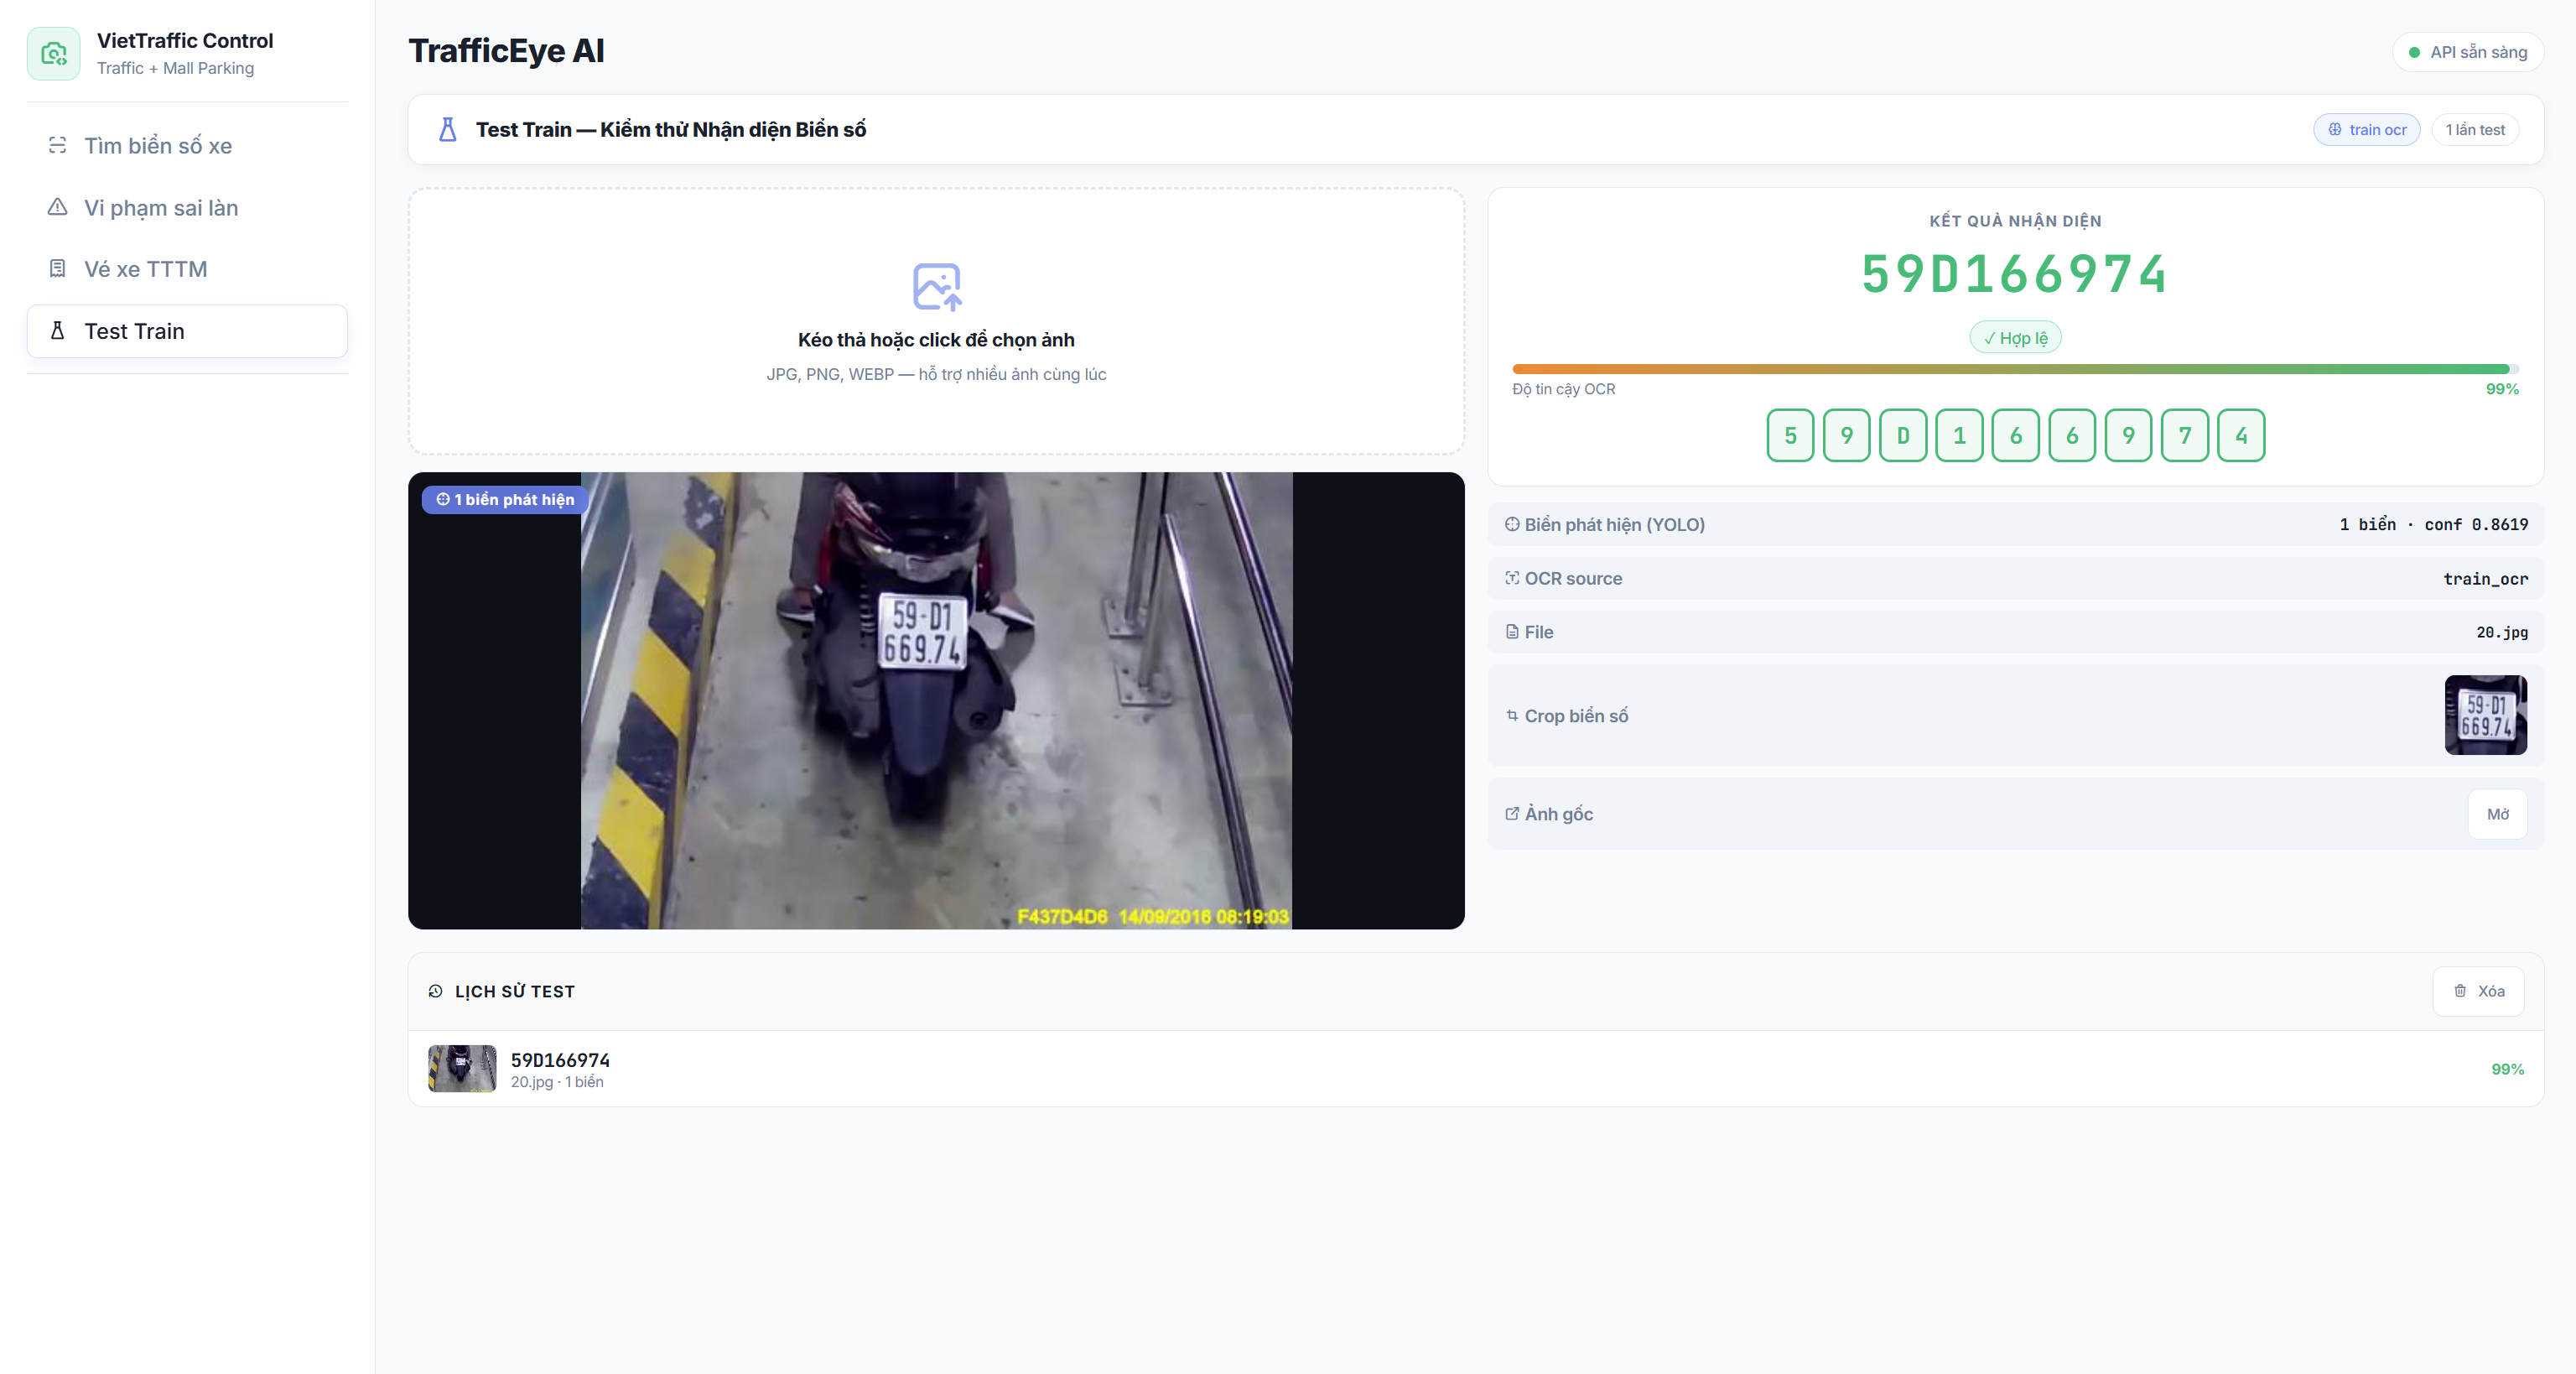
\includegraphics[width=\linewidth]{dashboard_detail.png}
\end{column}
\begin{column}{0.46\textwidth}
{\footnotesize Trang \textbf{Test Train}: tải ảnh \(\to\) YOLO cắt biển \(\to\) OCR đọc theo từng ký tự kèm độ tin cậy.}
\begin{table}\centering\scriptsize
\begin{tabular}{lll}
\toprule
\textbf{Thật} & \textbf{Đọc} & \\
\midrule
30G58236 & 30G58236 & Đúng \\
89LD00275 & 89LD00275 & Đúng \\
21A08531 & 21A08531 & Đúng \\
30E77379 & 30E77379 & Đúng \\
30F07555 & 30F03055 & \alert{Sai} \\
\bottomrule
\end{tabular}
\end{table}
{\scriptsize Ca sai chỉ lệch ở cụm số, mã tỉnh và chữ vẫn đúng.}
\end{column}
\end{columns}
\end{frame}

% ---------------------------------------------------------------
\begin{frame}{Phát hiện đi sai làn}
\begin{table}\centering\scriptsize
\begin{tabular}{llll}
\toprule
\textbf{Mã} & \textbf{Làn xuất phát} & \textbf{Hướng thực tế} & \textbf{Kết luận} \\
\midrule
CASE\_3 & Làn rẽ trái & Đi thẳng & Đi thẳng trên làn rẽ trái \\
CASE\_4 & Làn đi thẳng & Rẽ trái & Rẽ trái trên làn đi thẳng \\
CASE\_6 & Làn rẽ trái & Rẽ trái & Lấn làn đi thẳng rồi rẽ trái \\
\bottomrule
\end{tabular}
\end{table}
\begin{columns}[T]
\begin{column}{0.43\textwidth}
\begin{center}
\resizebox{!}{0.42\textheight}{%
\begin{tikzpicture}[font=\scriptsize,
  bx/.style={draw,rounded corners,align=center,text width=4.8cm,minimum height=0.6cm,inner sep=2pt},
  arr/.style={-{Latex[length=1.6mm]},semithick},node distance=2.6mm]
  \node[bx](a){Nạp cấu hình làn (đa giác)};
  \node[bx,below=of a](b){YOLOv8m + ByteTrack $\rightarrow$ quỹ đạo};
  \node[bx,below=of b](c){Điểm-trong-đa-giác $\rightarrow$ chuỗi vùng};
  \node[bx,below=of c](d){Xác định làn xuất phát + hướng};
  \node[bx,below=of d](e){Đối chiếu luật CASE\_3/4/6};
  \node[bx,fill=blue!12,below=of e](f){Vi phạm $\rightarrow$ xuất bằng chứng};
  \draw[arr](a)--(b);\draw[arr](b)--(c);\draw[arr](c)--(d);\draw[arr](d)--(e);\draw[arr](e)--(f);
\end{tikzpicture}}
\end{center}
\end{column}
\begin{column}{0.57\textwidth}
\textbf{Quy trình}
\begin{enumerate}\scriptsize
  \item Nạp cấu hình làn (đa giác làn + vùng hướng).
  \item Bám vết YOLOv8m + ByteTrack $\to$ quỹ đạo từng xe.
  \item Điểm-trong-đa-giác $\to$ chuỗi vùng (vd $1\!\to\!2\!\to\!4\!\to\!3$).
  \item Suy ra làn xuất phát \& hướng di chuyển thực tế.
  \item Đối chiếu luật (Nghị định 168/2024) $\to$ kết luận.
  \item Xuất ảnh bằng chứng, ghi cơ sở dữ liệu.
\end{enumerate}
{\scriptsize\textbf{Kết quả:} 141 vết, 2 vi phạm --- V001 xe máy (CASE\_6), V002 ô tô (CASE\_4).}
\end{column}
\end{columns}
\end{frame}

% ---------------------------------------------------------------
\begin{frame}{So sánh với hướng phát triển}
\begin{table}\centering\footnotesize
\begin{tabular}{lcccc}
\toprule
\textbf{Phương án} & \textbf{Seq/Plate} & \textbf{Char} & \textbf{CER} & \textbf{Điều kiện} \\
\midrule
Mô hình train (pipeline) & 75,39\% & 93,06\% & 6,96\% & Test, hậu xử lý \\
CRNN cơ sở & \textbf{83,10\%} & 95,68\% & 4,32\% & Test, thô \\
CRNN v2 (điều chỉnh tham số) & 93--95\%\,(dự kiến) & --- & \(\sim\)2,2\% & chưa đo \\
\bottomrule
\end{tabular}
\end{table}
\begin{columns}[T]
\begin{column}{0.5\textwidth}
{\footnotesize\textbf{Hướng phát triển = CRNN} (CNN+BiLSTM+CTC), gọn, hợp dữ liệu nhỏ.}
\begin{itemize}\scriptsize
  \item \textbf{v2} chỉ là \alert{điều chỉnh tham số} của CRNN cơ sở: lr, GroupNorm\(\to\)BatchNorm, dropout, label smoothing, lấy mẫu cân bằng, augment mạnh, SWA.
\end{itemize}
\end{column}
\begin{column}{0.5\textwidth}
\begin{itemize}\scriptsize
  \item Ở mức \textbf{thô}, CRNN (83,10\%) mạnh hơn train (51,31\%).
  \item 75,39\% của train là sau hậu xử lý, không so trực tiếp được.
  \item 93--95\% của v2 chỉ là dự kiến, chưa đo.
  \item \(\Rightarrow\) Hướng CRNN đáng theo đuổi tiếp.
\end{itemize}
\end{column}
\end{columns}
\end{frame}

% ---------------------------------------------------------------
\begin{frame}{Điểm mạnh, điểm yếu và nguyên nhân}
\begin{columns}[T]
\begin{column}{0.5\textwidth}
\textbf{Điểm mạnh}
\begin{itemize}\footnotesize
  \item Kiến trúc hiện đại, đa nhiệm.
  \item Train từ đầu, dễ tái lập.
  \item Tốc độ thời gian thực (\(\approx\)13 ảnh/s).
  \item Tích hợp pipeline đặc thù VN.
\end{itemize}
\end{column}
\begin{column}{0.5\textwidth}
\textbf{Điểm yếu}
\begin{itemize}\footnotesize
  \item Quá khớp (train 95\% vs val 51\%).
  \item Phụ thuộc nhiều vào hậu xử lý.
  \item Yếu ở nhóm khó \texttt{type2} (54\%).
  \item Chưa vượt CRNN ở mức thô.
\end{itemize}
\end{column}
\end{columns}
\medskip
\footnotesize\textbf{Nguyên nhân gốc:} độ phức tạp của Transformer lệch pha với quy mô dữ liệu nhỏ \(\Rightarrow\) phải bù bằng dữ liệu tổng hợp và hậu xử lý.
\end{frame}

% ---------------------------------------------------------------
\begin{frame}{Demo hệ thống --- giao diện web}
\begin{columns}[T]
\begin{column}{0.5\textwidth}
\centering
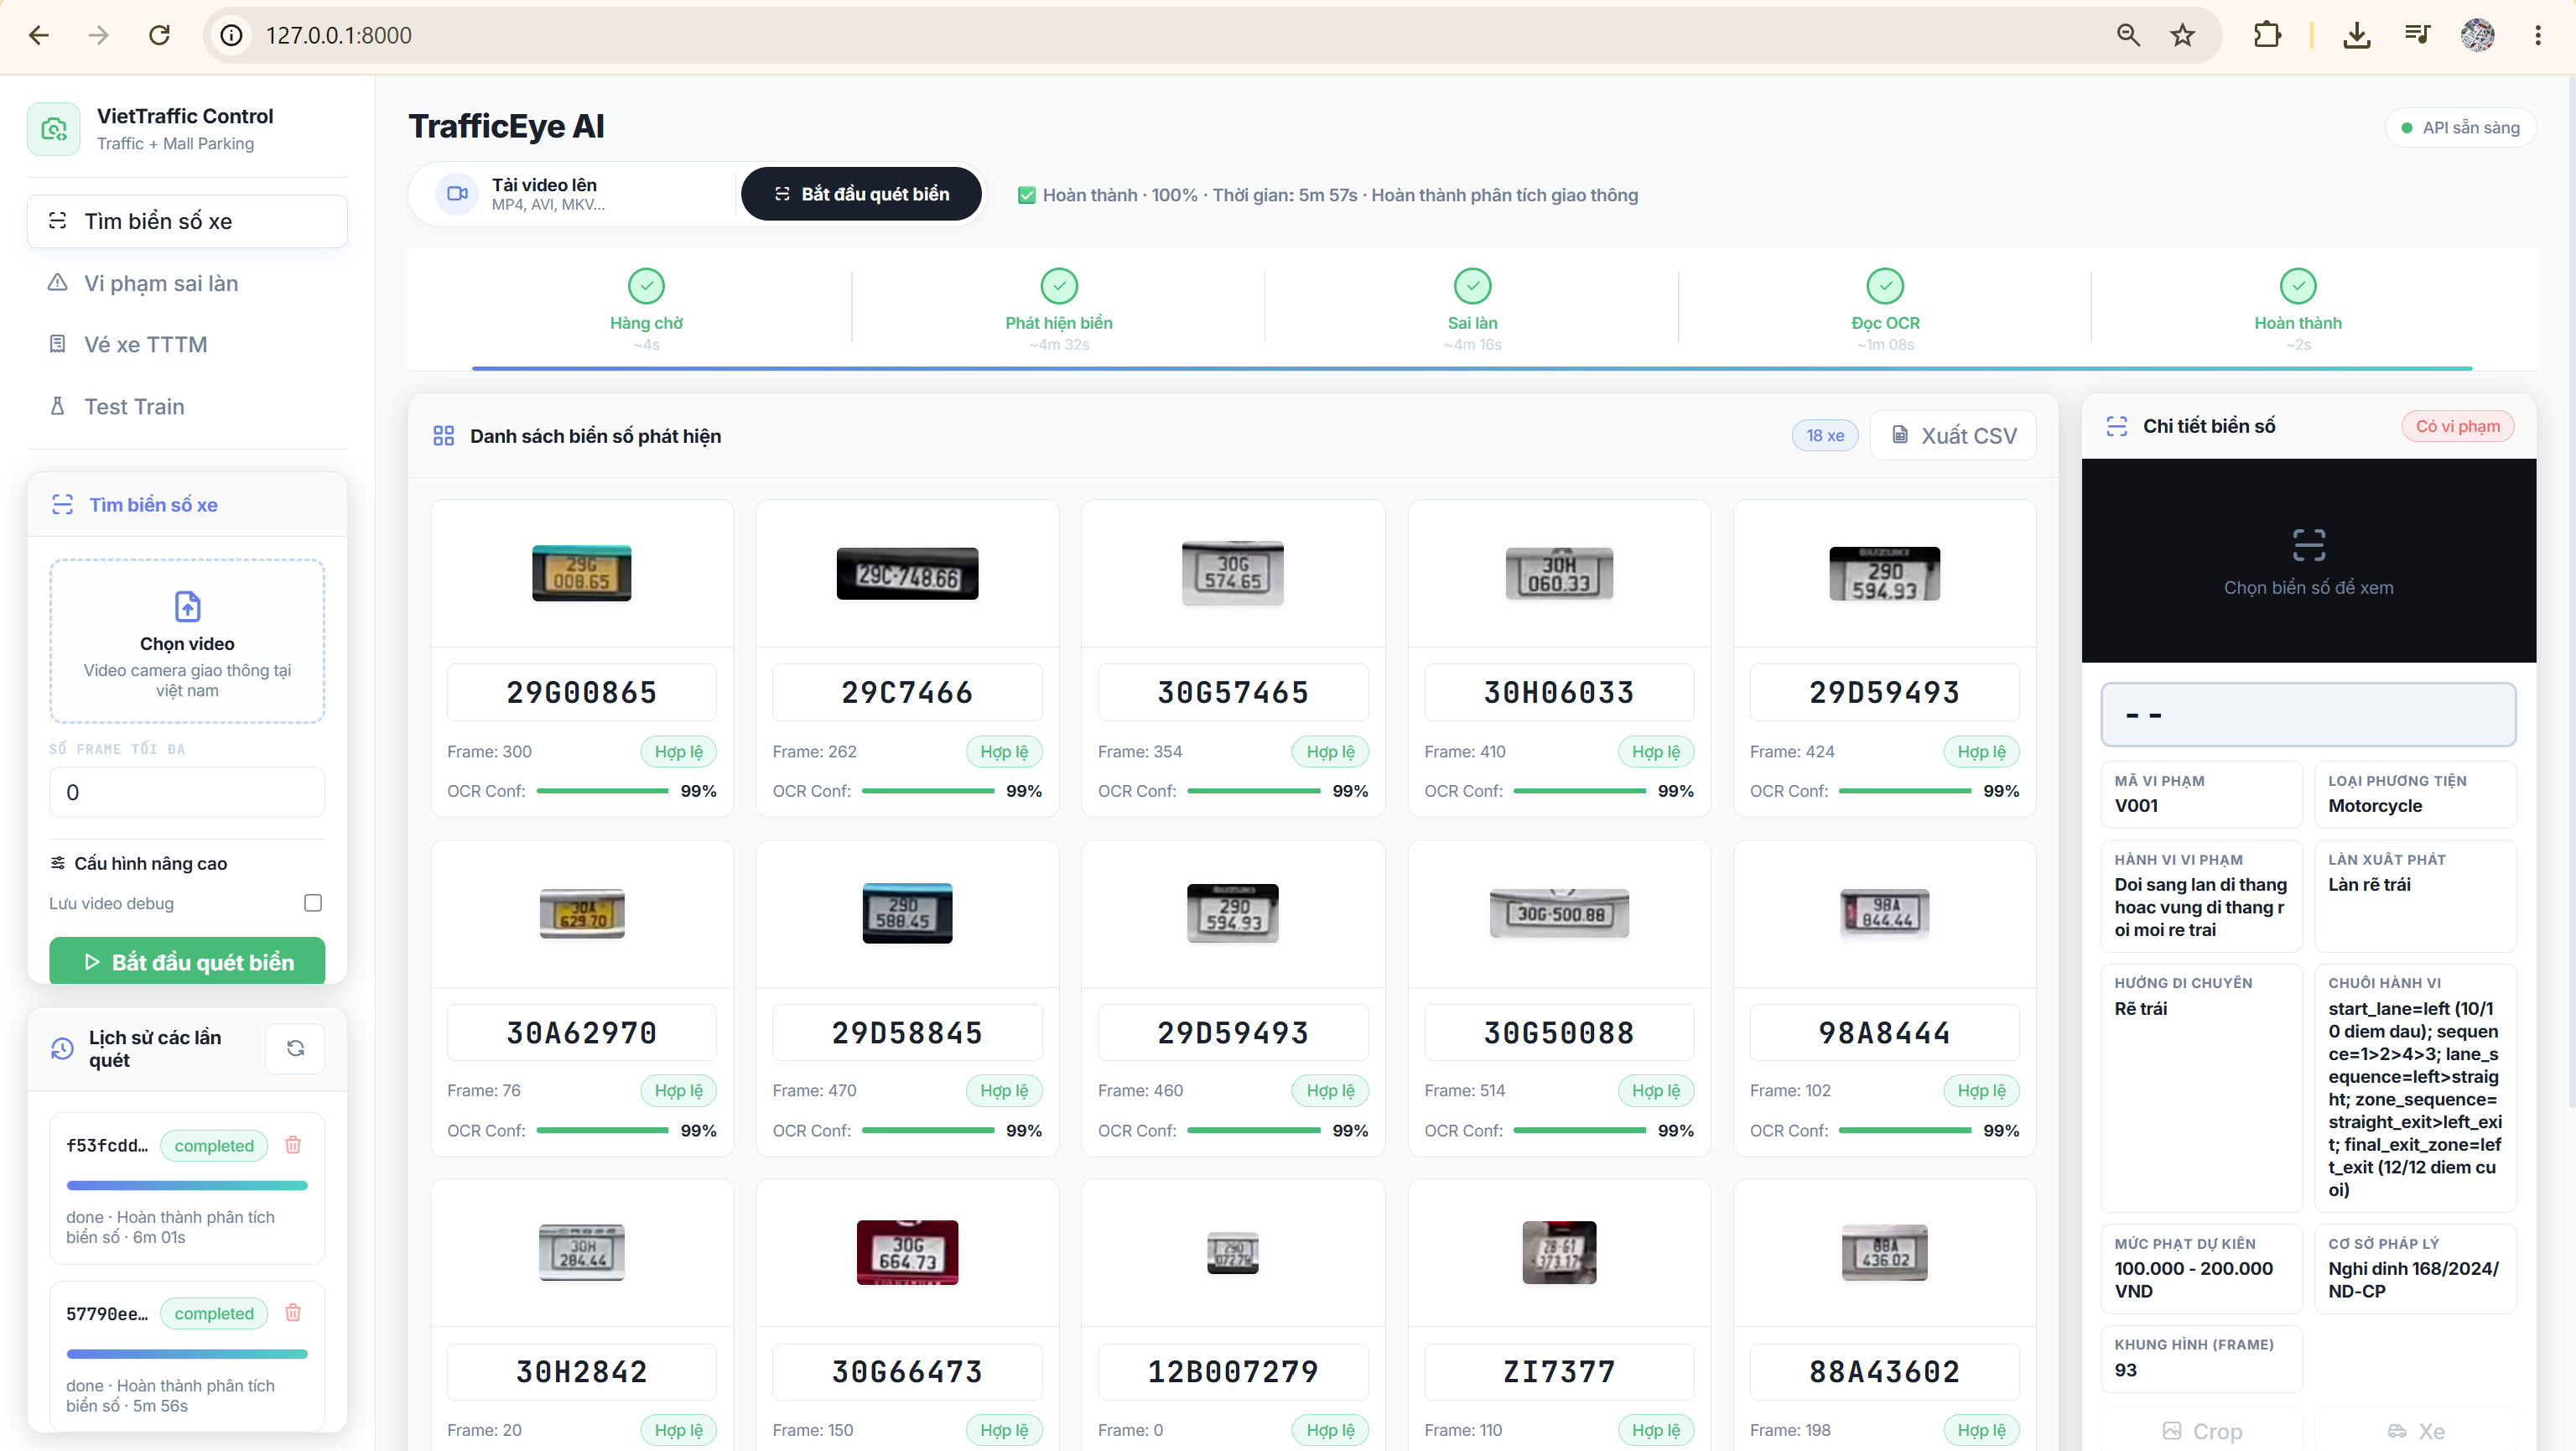
\includegraphics[width=\linewidth]{dashboard_live.png}\\[2pt]
{\scriptsize Trang \emph{Tìm biển số}: danh sách biển đã phát hiện kèm độ tin cậy.}
\end{column}
\begin{column}{0.5\textwidth}
\centering
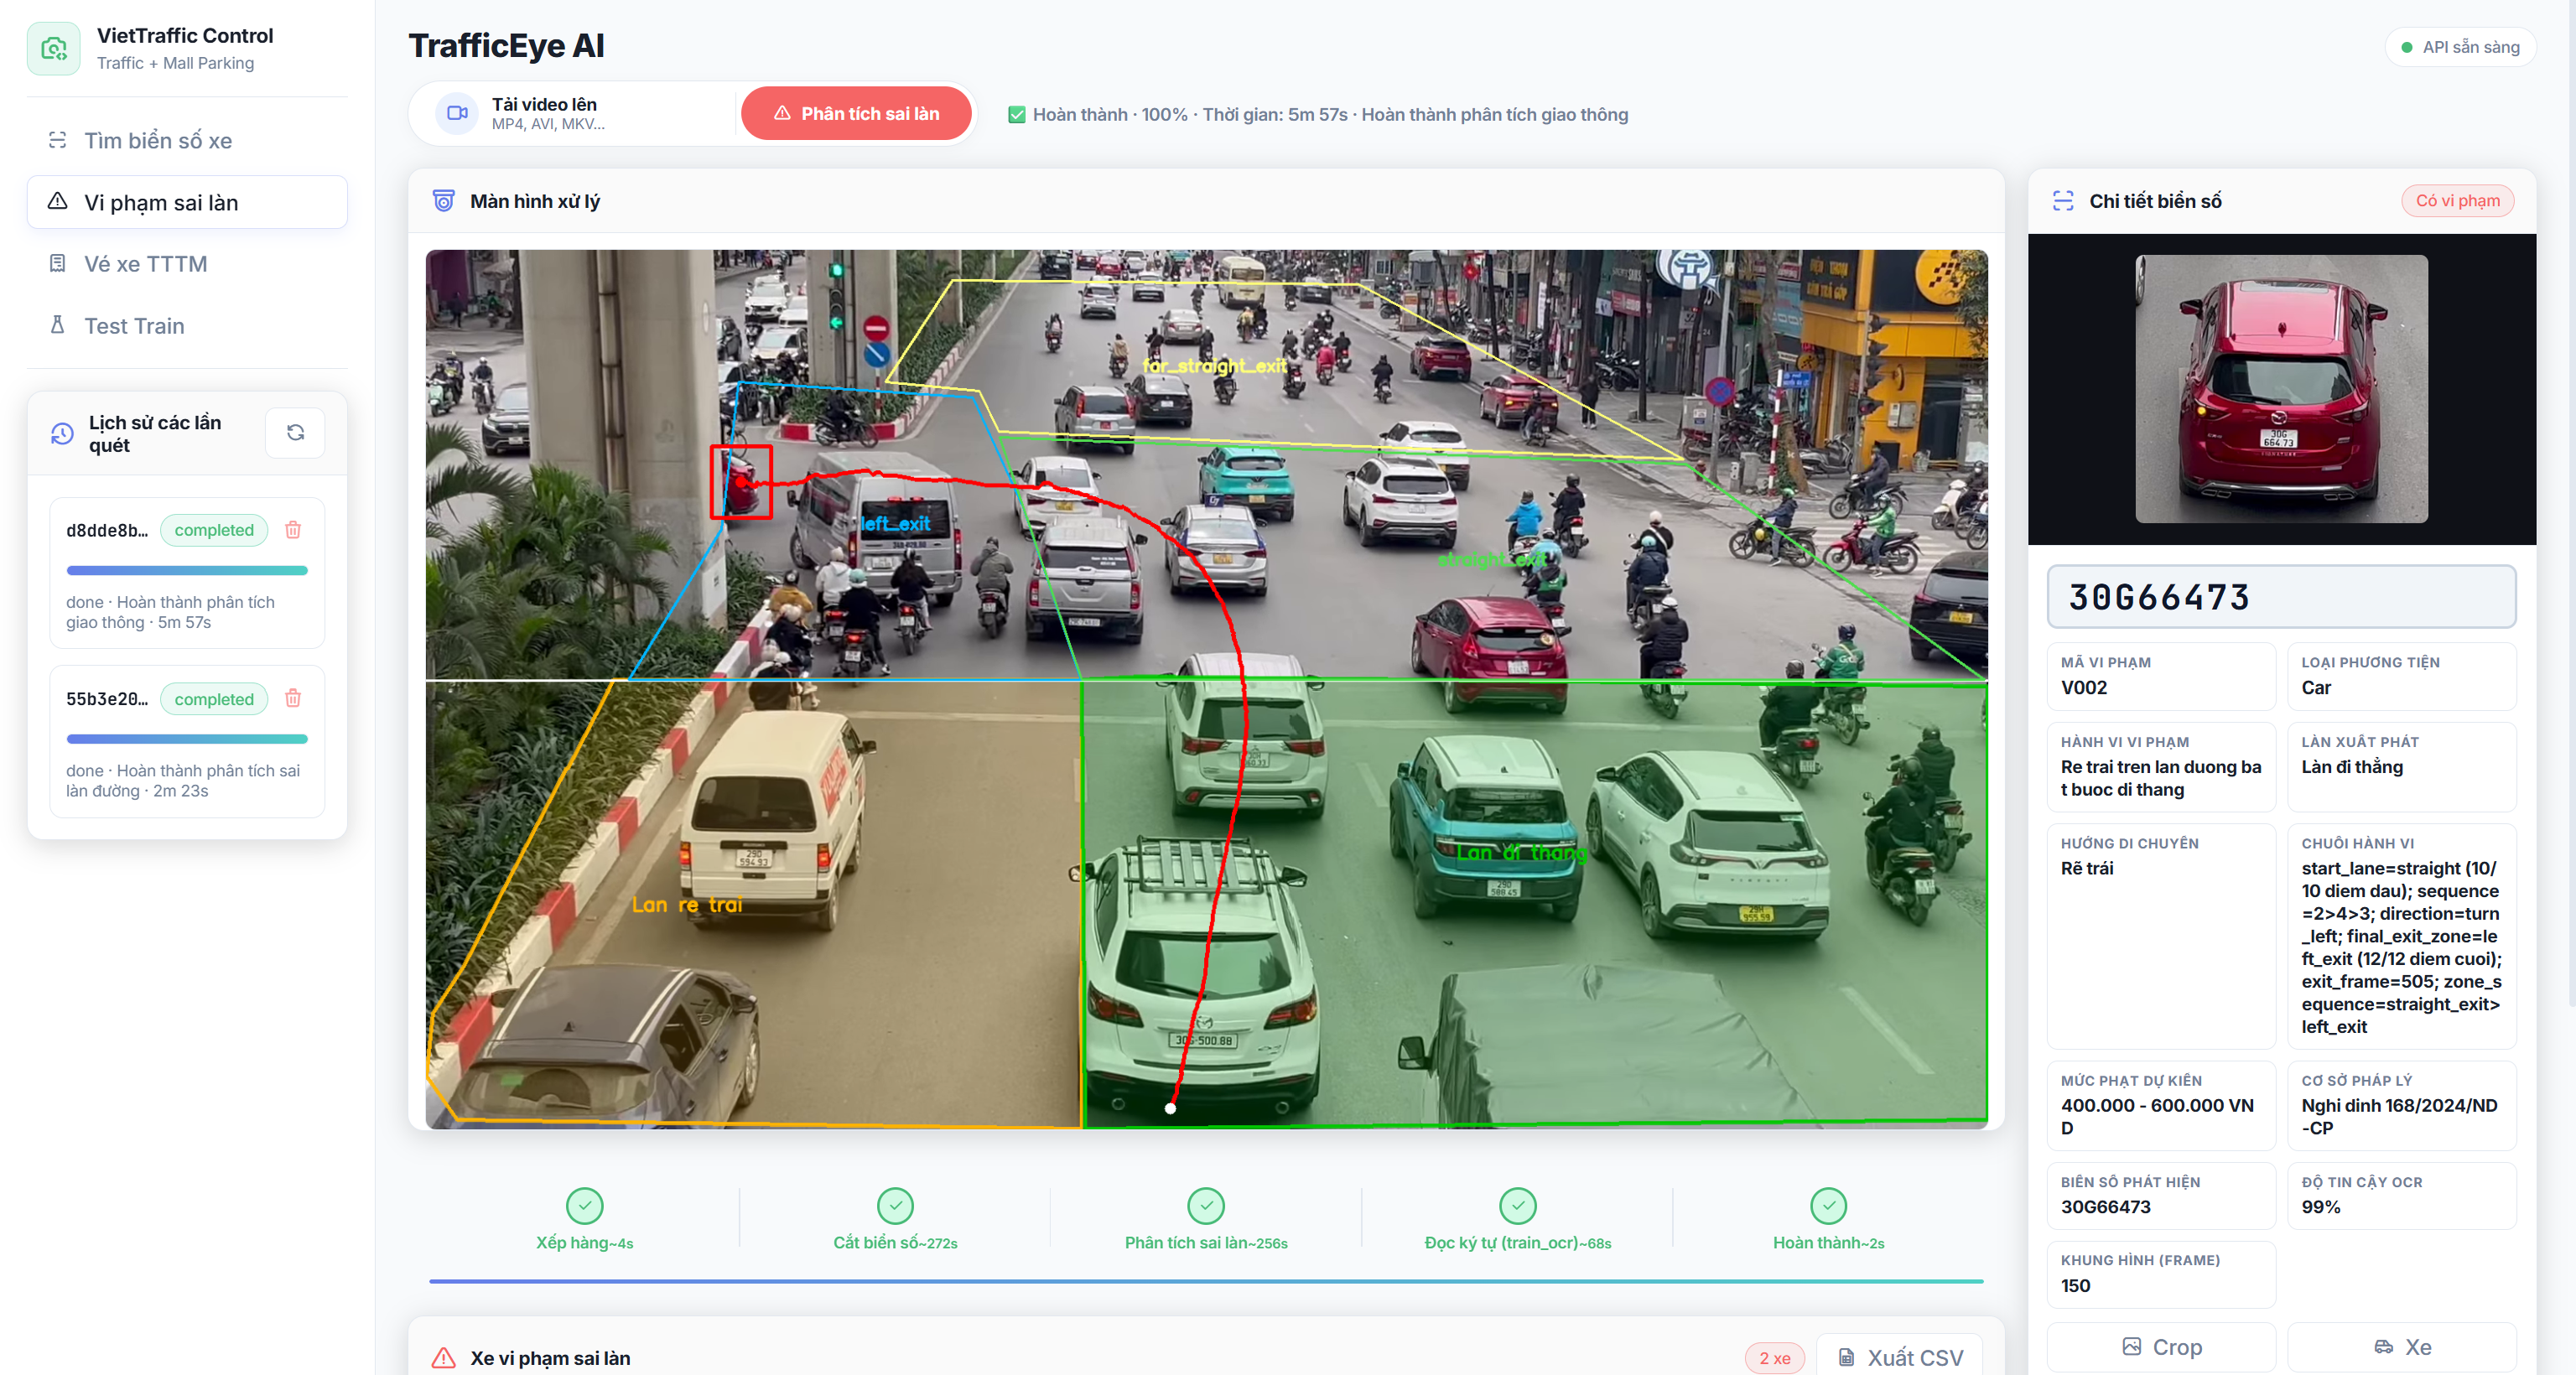
\includegraphics[width=\linewidth]{dashboard_list.png}\\[2pt]
{\scriptsize Trang \emph{Vi phạm sai làn}: phân tích làn trực tiếp + chi tiết xe vi phạm (biển số, lỗi, mức phạt).}
\end{column}
\end{columns}
\smallskip
{\footnotesize Kèm trang \textbf{Test Train} để tải ảnh và kiểm thử nhanh mô hình OCR.}
\end{frame}

% ---------------------------------------------------------------
\begin{frame}{Kết luận và hướng phát triển}
\textbf{Kết luận.} Mô hình OCR tự huấn luyện chạy trọn vẹn trong pipeline giám sát, đạt \textbf{93,06\%} ký tự / \textbf{75,39\%} toàn biển ở thời gian thực; còn dư địa cải thiện ở năng lực nhận dạng thô.
\medskip

\textbf{Hướng phát triển}
\begin{itemize}\footnotesize
  \item Giảm quá khớp: tăng điều chuẩn, giảm tỉ lệ ảnh tổng hợp, kiểm soát phân phối.
  \item Nâng năng lực thô: label smoothing, lấy mẫu cân bằng; theo đuổi hướng CRNN.
  \item Bổ sung dữ liệu cho nhóm khó (\texttt{type2}).
  \item Tối ưu triển khai: ONNX/TensorRT cho thiết bị biên.
  \item Đánh giá mọi phương án trên cùng điều kiện đo.
\end{itemize}
\end{frame}

% ---------------------------------------------------------------
\begin{frame}[plain]
\centering\vfill
{\Huge\textbf{Cảm ơn thầy đã lắng nghe!}}
\vfill
\end{frame}

\end{document}
